\chapter{Introduction}
\label{sec:intro}
In the current years the number of Cyber-physical systems (CPSs) has drastically increased. This is mostly due to the emergence of the Internet of Things (IoT), as well as the existence of several user friendly kits, like the RaspberryPi or the Arduino. With this new trend new challenges are created in the monitoring and debugging of these devices. This is especially difficult for applications, where the sensors are deployed in a hard to reach area. In addition to this, the deployed device can often fulfil a multi-purpose role and might need to be reconfigured for different tasks.

In order to address both these problems SHAMPU(Single chip Host for Autonomous Mote Programming over USB)\cite{Smeets:2014:DAL:2602339.2602401} was developed at the University Duisburg-Essen. SHAMPU was designed with the goal of being as small, lightweight and energy efficient as possible. In order to use SHAMPU as a test bed, it needs to be attached to an existing node. SHAMPU is then capable to not only monitor and debug the attached node, but also to program it. These reprogramming capabilities make it possible to reprogram an attached sensor, without having to physically be near it. To achieve this each SHAMPU node is equipped with a wireless interface. In the current configuration an ANT\cite{DynastreamInnovationsInc.2013} radio chip. All SHAMPU nodes form a Wireless sensor network (WSN) of their on, which allows not only the communication between the nodes, but also a connection to a base station. This base station not only acts as a central data sink for the whole network, but is also able to push commands and data to the SHAMPU nodes.

In this thesis we evaluate the wireless capabilities of the SHAMPU framework. For this purpose we develop use-cases for the different tasks that the SHAMPU framework can perform: Program a device, collect data during operation and interact with the system itself during runtime. For each of the test cases we design and run different experiments with the goal to assess if the chosen wireless technology is able to fulfil all the use cases.

\section{Related work}
\label{sec:related_work}
There are already several different WSN test beds available. Each of these test beds were designed to fulfil a different role. 

Some test beds like FlockLab \cite{Lim2013} allow to attach a wide array of different sensors and use a JTAG interface to be able to precisely capture debugging and timing information.
 
However, these types of test beds rely on a wired connection to interface with the test bed itself. That makes it exceedingly difficult to test and debug already deployed WSN, since it might not be possible to easily get to the sensor in the planted location.

Other available solutions address this problem by attaching the test bed directly to the node and use a wireless connection to communicate with the test bed. An example for this is Sensei-UU \cite{Rensfelt2009} which uses a wireless 802.11 network. This allows the WSN to be tested and debugged while it is deployed. One drawback of this solution is the power draw of 802.11 devices, which is huge, compared to other technologies. If the node itself is run of an external power source that isn't a problem, but the use of a battery to power the node will hardly be feasible.

To address this power issue, it is possible to use a different technology which offers a lower power mode. Two examples for this are BTNodes \cite{Moser} or Smart-Its \cite{Kasten2000}, which use a Bluetooth connection. 
The structure of the network itself is similar to Sensei-UU: each node in the network has its own test bed attached and the test beds communicate with a central base station.

The main problem with Bluetooth is the limited size of the network, which makes it difficult to set up and use more complex network topologies. Also Bluetooth communication is always 1:1 and does not allow broadcasts. The newest version of Bluetooth addresses the network size with the introduction of ScatterNets, but the setup and maintenance of the network still remains challenging.

\chapter{Technical Background}
\section{SHAMPU}
SHAMPU (Single chip Host for Autonomous Mote Programming over USB) \cite{Smeets:2014:DAL:2602339.2602401} is a WSN testbed which allows remote debugging and reprogramming of sensor nodes. Its main advantages over other testbeds (see section~\ref{sec:related_work}) are portability, low cost, small size and low energy consumption. SHAMPU is used as an extension to an already existing sensor node. The only requirement is that the node provides an USB-Interface which is connected to SHAMPU. This single connection to the attached node makes SHAMPU completely OS independent.
\begin{figure}[H]
\centering
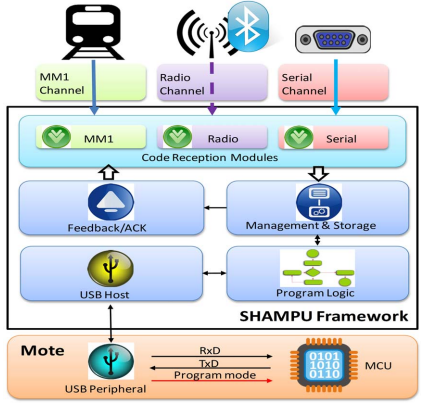
\includegraphics[scale=.5]{./pics/SHAMPUframework.png}
\caption{Overview of the SHAMPU Framework \cite{Smeets:2014:DAL:2602339.2602401}}\label{fig:shampuframework}
\end{figure}
The SHAMPU framework (see Figure \ref{fig:shampuframework}) itself is split into multiple modules. The most important part for this thesis is the Code Reception Module, which allows the use of different protocols to connect to and communicate with the SHAMPU device. One option for the wireless communications with the SHAMPU device is the ANT protocol, on which we will focus in this evaluation.

\section{ANTAP1MxIB RF}
In order to use the ANT protocol each SHAMPU-mote is equipped with an ANTAP1MxIB RF Transceiver Module. The module was chosen because of its small form factor (20mm x 20mm) and its very low power draw. The ANTAP1M can handle up to 4 different ANT channels with a combined message rate which ranges between 0.5Hz and 200 Hz. 

\begin{figure}[H]
	\centering
	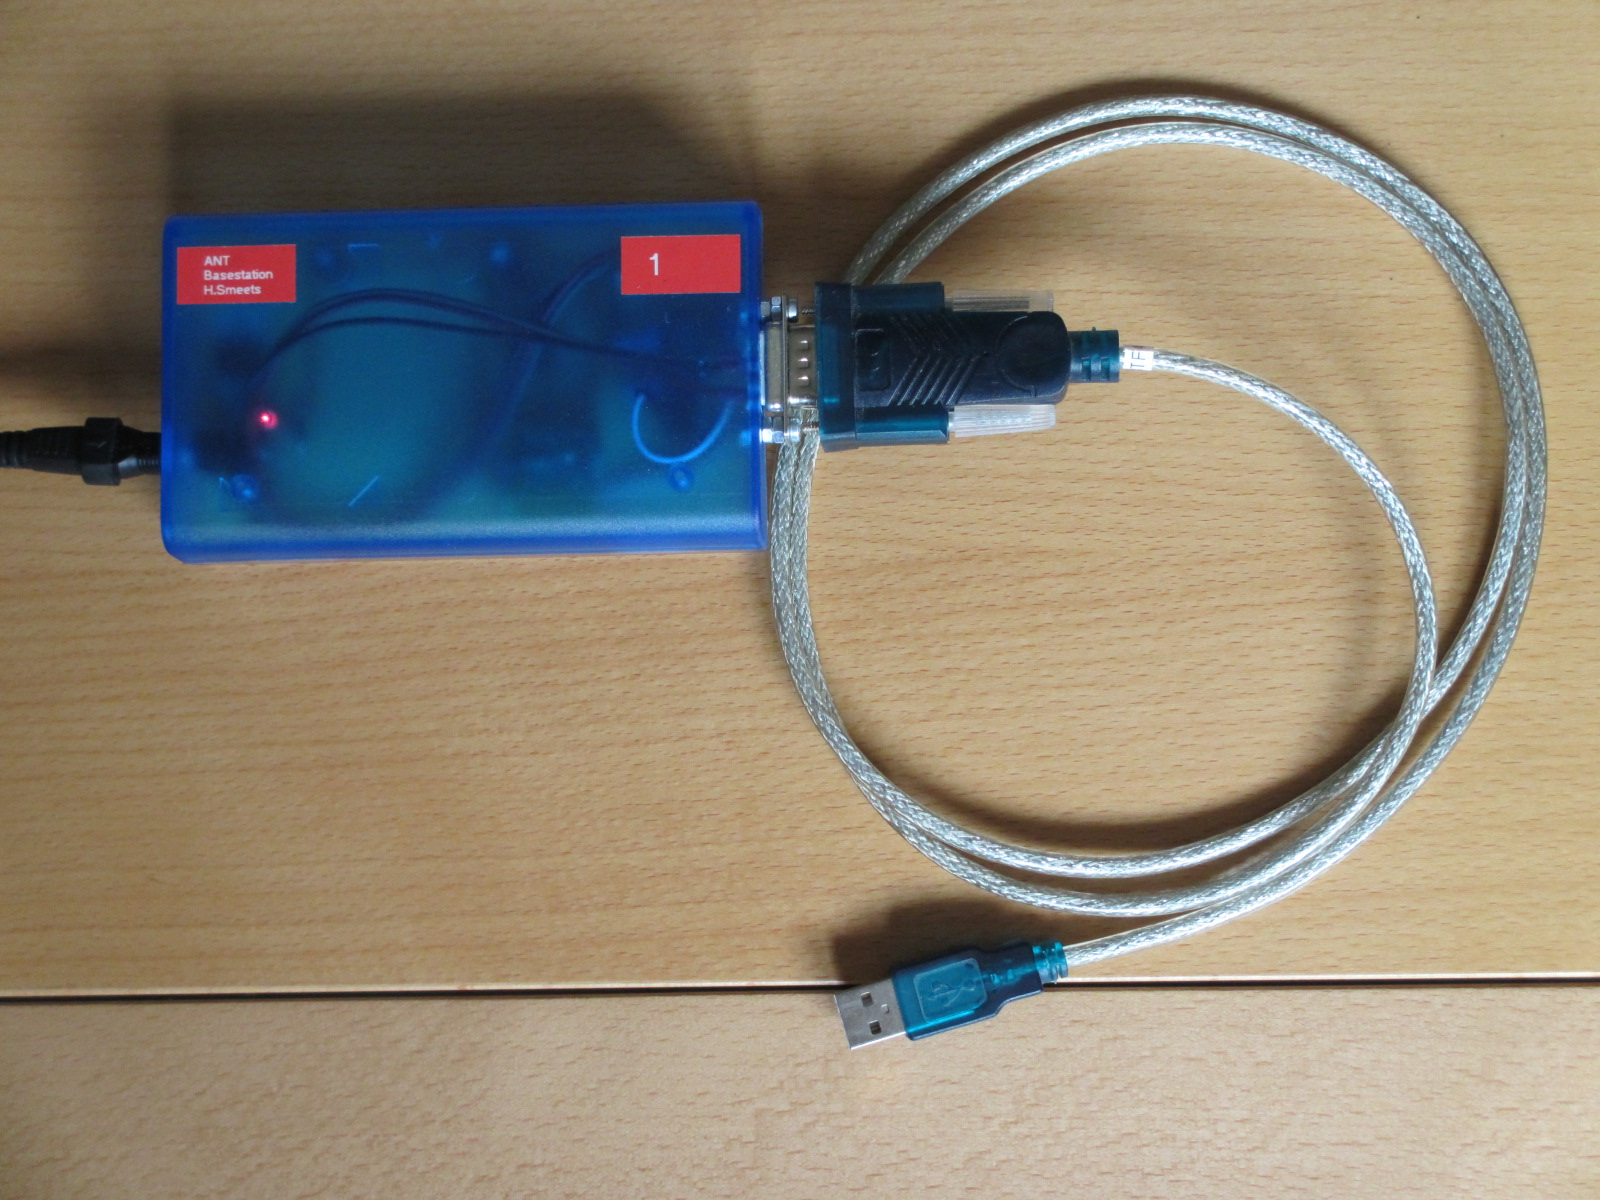
\includegraphics[scale=.5]{./pics/SHAMPUbase.JPG}
	\caption{SHAMPU base station}\label{fig:shampubase}
\end{figure}
In order to more easily test the capabilities of the ANT chip, we use a SHAMPU base station for all the experiments. This base station (see Figure \ref{fig:shampubase}) contains the ANTAP1MxIB and a serial interface, which allows the ANT to asynchronously communicate with a PC over RS-232. 

\section{ANT}
ANT \cite{DynastreamInnovationsInc.2013} is a wireless protocol which operates in the 2.4 GHz ISM Band. It was originally developed in 2003 by Dynastream Innovations Inc. for the use in wireless sensors. The ANT protocol is designed for the use in low power WSNs focusing on scalability and ease of use.

One of the advantages ANT has over other protocols, such as Bluetooth or ZigBee, is the high level of abstraction the ANT Protocol provides. 
\begin{figure}[H]
	\centering
	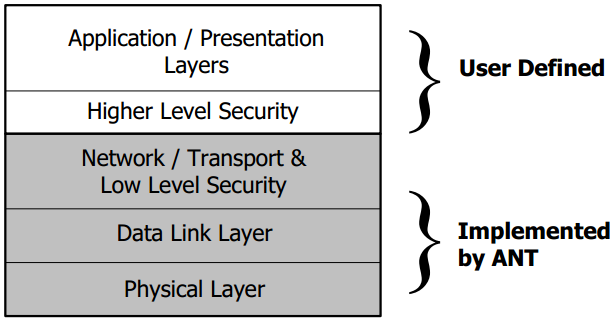
\includegraphics[scale=.5]{./pics/ANTstack.png}
	\caption{OSI-Layer vs. ANT Protocol\cite{Networks}}\label{fig:osilayer}
\end{figure}

This level of abstraction is achieved by incorporating the first 4 OSI-layers (see Figure \ref{fig:osilayer}) into the ANT protocol, thus allowing even low-cost MCU to set up and maintain complex wireless networks, since all the details of the communication are handled by the ANT-chip.

\subsection{ANT Topology}
In order for the ANT protocol to work each mote needs to be part of a network. As shown in figure \ref{fig:anttopo} the ANT protocol can be used to create simple or considerably more complex networks. Each mote inside a network is called an ANT node. In order for two nodes to communicate with each other they need to be connected via a channel.

\begin{figure}[h]
	\centering
	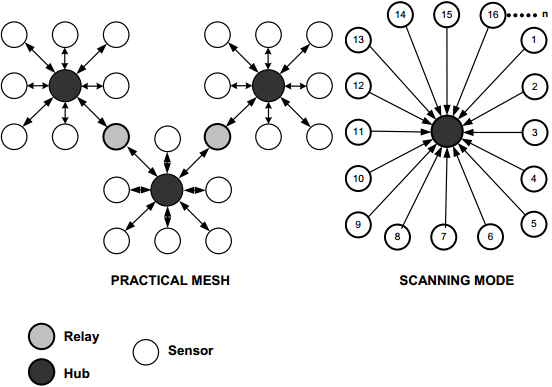
\includegraphics[scale=0.7]{./pics/ANTtopo.png}
	\caption{Example ANT Topologies\cite{DynastreamInnovationsInc.2013}}\label{fig:anttopo}
\end{figure}

\subsection{ANT Channels}
Most of the available channel types are bidirectional. The ANT protocol, however, still differentiates between master and slaves nodes. While a master node mostly sends data and a slave node mostly receives data, the slave retains the ability to respond to the incoming data.

The ANT protocol knows 125 different channels, each of them 1 MHz wide. Each Channel can support a data rate of 1 Mbps and up to 65533 nodes. To avoid interference between the channels isochronous self adjusting TDMA technology is used, which allows the ANT nodes to change the transmit timings as well as the frequency that is being used for the current channel. The use of the TDMA is completely handled by the ANT protocol, which means the user has no control over the process.

\begin{figure}[H]
	\centering
	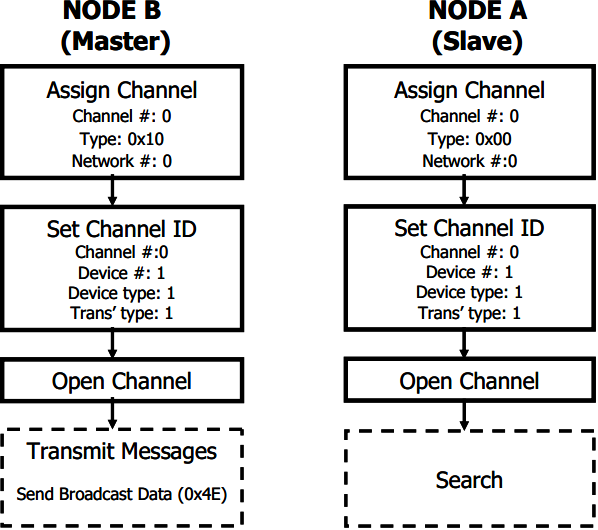
\includegraphics[scale=0.7]{./pics/ANTsetup.png}
	\caption{ANT Channel Establishment\cite{DynastreamInnovationsInc.2013}}\label{fig:antsetup}
\end{figure}

Figure \ref{fig:antsetup} shows the procedure of opening up a channel between two ANT nodes. In the first step the Channel configuration is set, most important in this context being the channel type: 0x00 signifies that the node is a slave while 0x10 means that the node acts as a master. The next step is to set the Channel ID. Here the slave node needs to set the values of the master device in order to correctly connect. It is possible, however, to set wildcard values, which allows the slave to connect to any device sending on the same frequency. Before the final step, it is optionally possible to set the frequency of the channel and the message period. These steps are not mandatory though, since ANT defaults to fixed values for these: 2466 Hz transmission frequency and a message period of 8192. The last step constitutes of the opening of the channel itself, where care should be taken that the master opens the channel before it is opened by the slave device.

The ANT protocol distinguishes between two different Channel types:
\begin{description}
\item{\textbf{Independent Channels}} \hfill \\ Independent Channels are used if there is only one node which transmits  data. There is no limit to the amount of slave devices which receive the messages that are being sent out. Furthermore, the message being sent out is broadcast to all nodes, it is not possible to address only specific nodes.
\item{\textbf{Shared Channels}} \hfill \\ Shared Channels are used if there is more than one node which sends data. This type of channel is facilitated by the use of a Shared Channel Address, which in turn reduces the amount of data that can be transmitted at a time. All ANT nodes still receive every message, but only forward messages which have a matching address. The Channel master can decide to either use one or two bytes as the address, which allows for either 255 or 65535 slave devices in the same channel. 
\end{description}

\subsection{ANT Communication}

The ANT protocol supports three different data types: broadcast, acknowledge and burst. The data type is not part of the channel configuration, thus channels are able to use any combination of data types. The only exceptions are unidirectional channels, which can exclusively send broadcast data. The various data types differ in the way data is handled and transmitted.

\begin{itemize}
	\item{Broadcast data} \hfill \\ Broadcast data represents the most basic data type and, at the same time, the default. To start a broadcast transmission, the command needs to be issued just once, since the last sent packet is periodically resent as a broadcast. It does not matter if the last packet was part of a burst or acknowledge transmission, if no new data is available this packet is resent. Figure (MISSINGPIC) shows, how each broadcast transmission is aligned to the channel message period.	Since there is no answer from the receiving node, it is not possible to determine if the packet was transmitted correctly.

	\item{Acknowledge data} \hfill \\ Acknowledge data can be used to make sure a node has received a transmitted packet. After receiving an acknowledge packet the node will send a message back to the sender. Acknowledge data can only be used with bidirectional channels, yet both the master and the slave can use it. Figure (MISSINGPIC) shows that, just like broadcast data, acknowledge data is always aligned to a time slot, yet the answer from the receiver is sent immediately back to the sender.
	
	\item{Burst data} \hfill \\ Burst data provides a method to quickly transmit large amounts of data. This is achieved by ignoring the normal channel time slots and sending the packets immediately one after the other. This allows for a transmission rate of up to 20 kbps, which is much higher than other data transmission types. Similar to acknowledge data at the end of the transmission the sender is informed if the transfer failed or succeeded. The drawback of this method is, that burst data is prioritized over all other transmissions and will interrupt other transmissions over the same channel.
\end{itemize}

\subsection{ANT messages}
In the ANT protocol each message has the basic format as specified in Figure \ref{fig:antmsg}.
\begin{figure}[h]
	\centering
	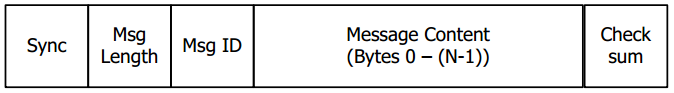
\includegraphics[scale=.75]{./pics/ANTmsg.png}
	\caption{Ant message structure\cite{DynastreamInnovationsInc.2013}}\label{fig:antmsg}
\end{figure}
Each message starts with a special Sync-Byte and ends with a checksum, which is calculated by xoring all previous bytes. The Msg Length byte is the number of Message Content bytes. The Msg ID byte specifies which kind of data is contained in the message. The ANT protocol also provides an extended message format, which allows to attach further information to each message. The maximum length of the message content is 8 for each of the three data types.

\chapter{Evaluation of SHAMPU}
In order to assess the capabilities of SHAMPU, we plan and run experiments designed to evaluate the SHAMPU framework according to the following use-cases:
\begin{itemize}
	\item{\textbf{Scheduled data-transmission}} \hfill \\ In order for SHAMPU to work as a debugging and logging platform, the base station needs to periodically receive data from all the nodes in the network. ANT provides two different data types which can be used to transport data in this case: Broadcast data and Acknowledge data. The experiments designed for this use case try to determine the maximum throughput for each of the two transfer modes.
	\item{\textbf{Unscheduled data-transmission}} \hfill \\ There are several possible cases, where it is not feasible to use a scheduled data-transmission. Instead, the burst mode must be used, which allows to transmit data at a much higher rate. This use case covers several different scenarios, e.g.:
	\begin{itemize}
		\item{}Reprogramming of a node: SHAMPU is able to reprogram the attached node. For this process, SHAMPU needs to receive a new firmware, which can amount to several hundred kB.
		\item{}SHAMPU RAM-Dumps: SHAMPU has 128kB of RAM, which can be used to save collected data during an experiment. At the end of the experiment the complete memory needs to be transmitted back to the base station.
	\end{itemize}
	\item{\textbf{Communication range}} \hfill \\ Since SHAMPU is architecture independent it can be used in different situations. Therefore it is important to know, how far away from the base station the nodes can be placed. As SHAMPU tries to be energy efficient, it might also be viable to reduce the range for smaller set ups to save even more energy.
\end{itemize}

To cover all the mentioned test cases we designed different experiments, which test one or more of the described categories. The following section describes the experiments according to the following template:

\begin{description}
\item{\textbf{Description}} \hfill \\ A description of the experiment and the category being evaluated.
\item{\textbf{Use-Case}} \hfill \\ The use-case which the experiment tries to test.
\item{\textbf{Network Topology and Configuration}} \hfill \\ A diagram of the network topology in which the experiment is run and pseudo code which describes the program being run on the master and the slave. Default values are not listed.
\item{\textbf{Testing methodology}} \hfill \\ A description how the experiment is performed.
\item{\textbf{Result}} \hfill \\ The results of the experiment and any additional data collected during the experiment.
\end{description}

\newpage

\section{Common experiment parameters}
\begin{figure}[h]
	\centering
	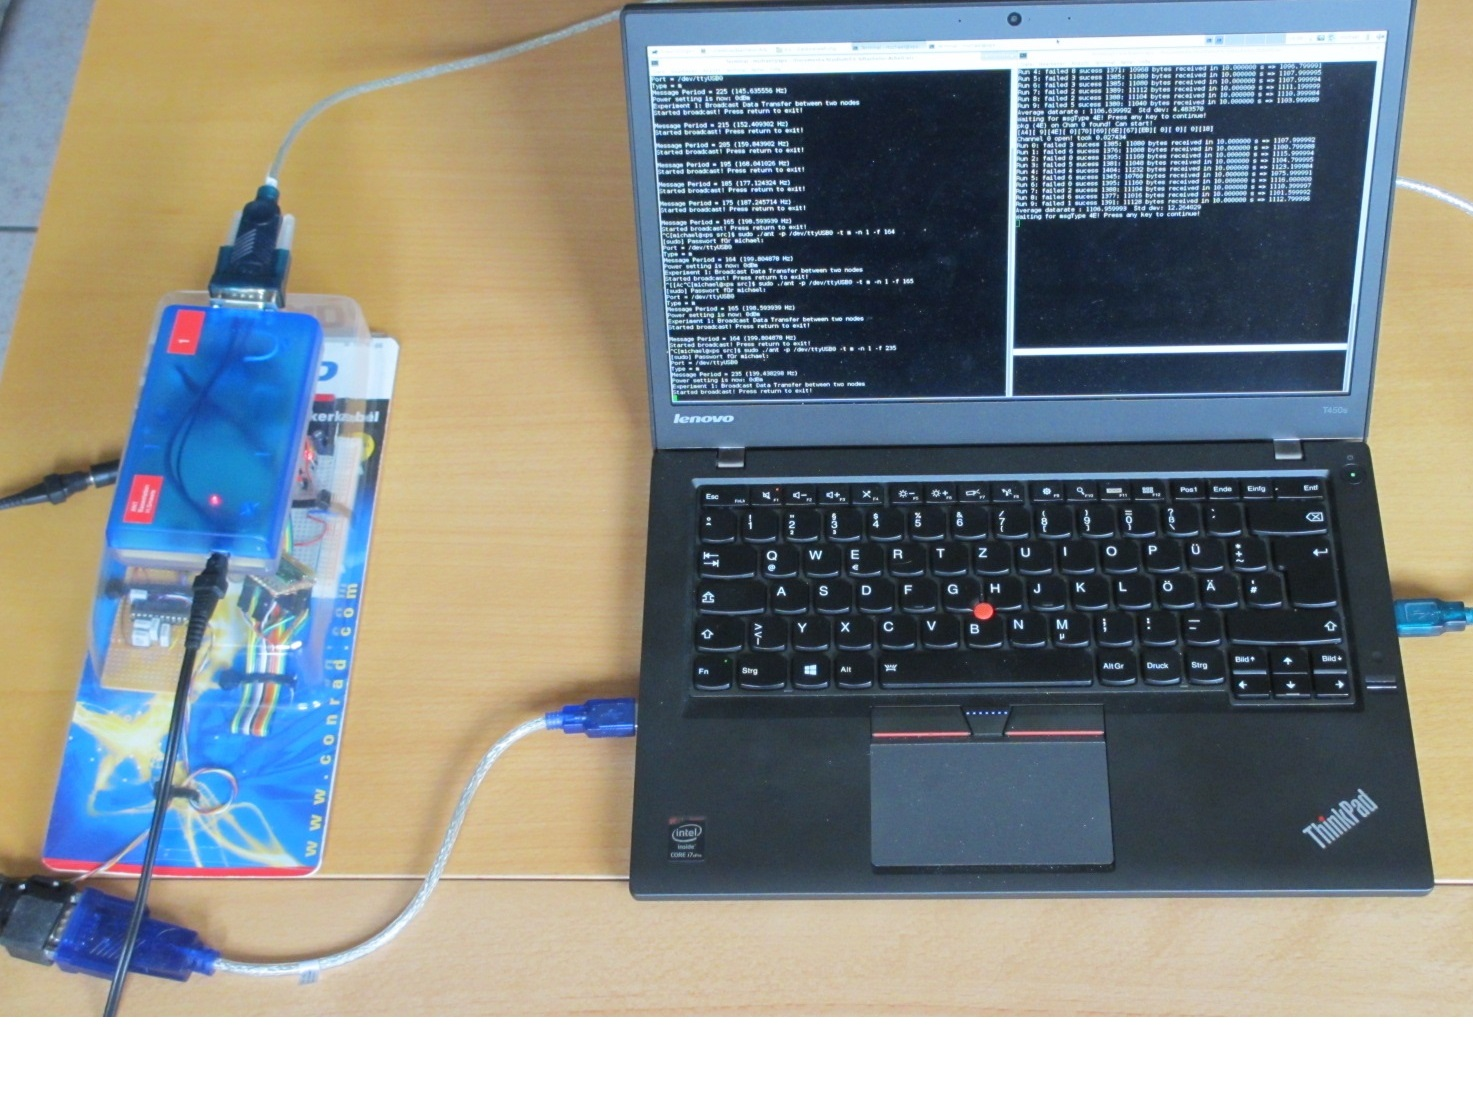
\includegraphics[scale=.75]{./pics/expSetup.JPG}
	\caption{Experiment set up}\label{fig:expSetup}
\end{figure}

If not otherwise noted in the experiment description each experiment was run in the Mobility Lab of the Networked Embedded Systems group at the University of Duisburg-Essen (SA 327), with the two base stations in the configuration which can be seen in figure \ref{fig:expSetup}. The following table describes the parameters which are used in the experiments.
\begin{center}
\begin{tabular}{|c|c|}
	\hline Device Number & 33 \\ 
	\hline Device Type & 1 \\ 
	\hline Transmission Type & 1 \\ 
	\hline ID\_CHAN1 & 0 \\ 
	\hline FREQ\_CHAN1 & 2466 Hz \\ 
	\hline ID\_CHAN2 & 1 \\ 
	\hline FREQ\_CHAN2 & 2477 Hz \\ 
	\hline Message Period & 8192 \\ 
	\hline min\_Channel\_Period & 0x00A5 \\ 
	\hline max\_Channel\_Period & 0xFFFF \\ 
	\hline 
\end{tabular} 		
\captionof{table}{ANT default configuration}
\end{center}

Also, there is an important difference between the message period used in the pseudo code and the frequency used in the figures which display the results. The period describes the size of the gap between two messages, the frequency describes how many messages are sent in 1 second. The channel period $p$ can be used to calculate the frequency of the time slots $f_t = \frac{32678}{p}$.  
\newpage

\section{Experiment 1: Broadcast Data Transfer between two nodes}
\begin{description} 
	\item{\textbf{Description}} \hfill \\ Broadcasting is one way of periodically transmitting data between two or more ANT nodes. Since all broadcast packets are synchronized to a fixed time-slot, the data throughput can be increased by decreasing the channel period. The experiment itself is split into two parts. In the first part we try to determine the highest possible data throughput. Also we try to determine if the channel period has an effect on the time it takes for a slave node to find and join an existing channel. The second part is a test of the highest detected data throughput. Here we try to evaluate if there are any variations of the data throughput over a much longer interval.	
	\item{\textbf{Use-Case}} \hfill \\ Scheduled Data-transmission	
	\item{\textbf{Network Topology and Configuration}} \hfill \\ 
	\begin{figure}[H]
		\centering
		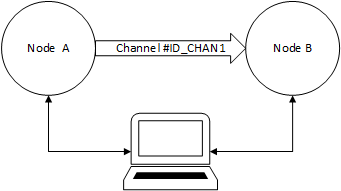
\includegraphics[scale=1]{./pics/exp_topo.png}
		\caption{Toplogy experiment 1}
	\end{figure}
		\begin{code}[H]
			\begin{verbatim}
			channelPeriod = max_Channel_Period
			while (channelPeriod >= min_Channel_Period) {
			  ANT_SetChannelPeriod(ID_CHAN1, channelPeriod)
			  ANT_OpenChannel(ID_CHAN1, ANT_Bidirectional_Master)
			  ANT_SendBroadcastData(ID_CHAN1, [0x01, 0x02, 0x03, 0x04])
			  wait_for_user_input()
			  ANT_CloseChannel(ID_CHAN1)
			  channelPeriod = decreaseChannelPeriod()
			}
			\end{verbatim}
			\caption{Broadcast data single channel (Master)}\label{lst:mExp1}
		\end{code}
		
		\begin{code}[H]
			\begin{verbatim}
			channelPeriod = max_Channel_Period
			while (channelPeriod >= min_Channel_Period) {
			  for (i in 0..9) {
			    ANT_SetChannelPeriod(ID_CHAN1, channelPeriod)
			    ANT_OpenChannel(ID_CHAN1, ANT_Bidirectional_Slave)
			    count = 0
			    for (100 seconds) 
			      if (receivedPacket() == ANT_BROADCAST_DATA)
			        count++;			  
			    print (count * 8 / 100) + " Bytes per second"
			    wait_for_user_input()
			    ANT_CloseChannel(ID_CHAN1)
			  }
			  channelPeriod = decreaseChannelPeriod()
			}
			\end{verbatim}
			\caption{Broadcast data single channel (Slave)}\label{lst:sExp1}
		\end{code}	
	\item{\textbf{Network Topology and Configuration}} \hfill \\ The 2 nodes are placed right next to each other.
	 \item{\textbf{Testing methodology}} \hfill \\Node A acts as the master and node B as the slave. For both nodes the channel period is set to the highest value and the channel is opened. Node B records how long it takes to join the channel and how many bytes it received over a 100s interval. The measurement is repeated 10 times and the average values are saved. Then the channel period is decreased and the process is repeated. For the second part, the channel period is set to the value which achieved the highest speed. The experiment is then left running for a period of 10 hours in one continuous run.
	\item{\textbf{Result}} \hfill \\  
	\begin{figure}[H]
	\centering
	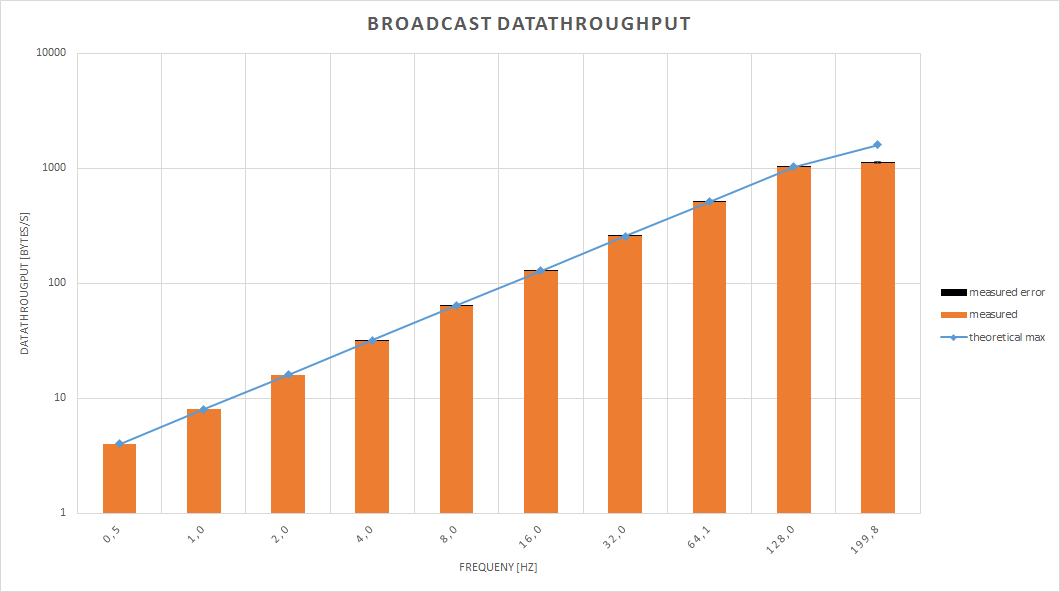
\includegraphics[scale=0.5]{./pics/exp1_norm.png}
	\caption{Broadcast data rate (0.5Hz - 128Hz)}\label{fig:exp1norm}
	\end{figure}
	
	Figure \ref{fig:exp1norm} shows the transmission speeds achieved for the different frequencies. Up to a frequency of 128 Hz, the measured data rate matches the expected theoretical maximum rate. For the highest supported frequency (199.8 Hz), the measured data rate is much lower than the maximum rate. Even if we account for transmission errors the difference is significant. 
		\begin{figure}[H]
			\centering
			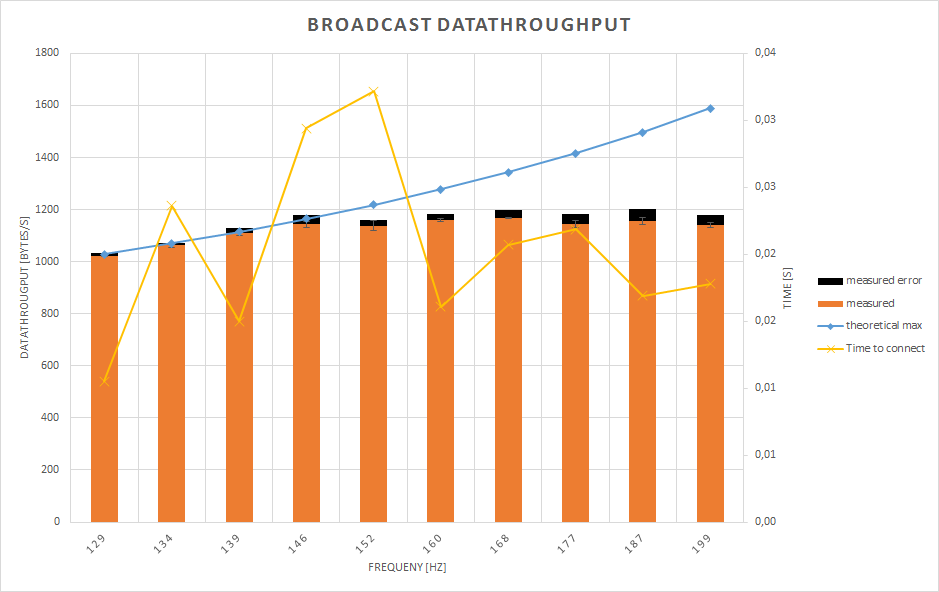
\includegraphics[scale=0.5]{./pics/exp1_detail.png}
			\caption{Broadcast data rate (129Hz - 199Hz)}\label{fig:exp1between}
		\end{figure}
	As seen in figure \ref{fig:exp1between} the measured data rates for frequencies above 140 Hz all fall short of the expected values. However the average data throughput of these frequencies remains consistently at around 1100 Bps. The experiment was repeated multiple times, running it at different times and places, thus an environmental factor can be excluded. That means, the reason for the upper limit has to be found with the hardware itself. See section \ref{sec:dataThrougput} for a discussion about possible reasons for this upper limit.
	
	The time it takes for a Node to join a channel falls rapidly once the frequency is above 1 Hz. For frequencies above 64 Hz, the time it takes to join a channel becomes negligible, with times around 75 ms (see Figure \ref{fig:exp1norm}). All the measured values are below the specified worst case channel acquisition times of the ANT protocol \cite{AntChan}.
	
	\begin{figure}[H]
		\centering
		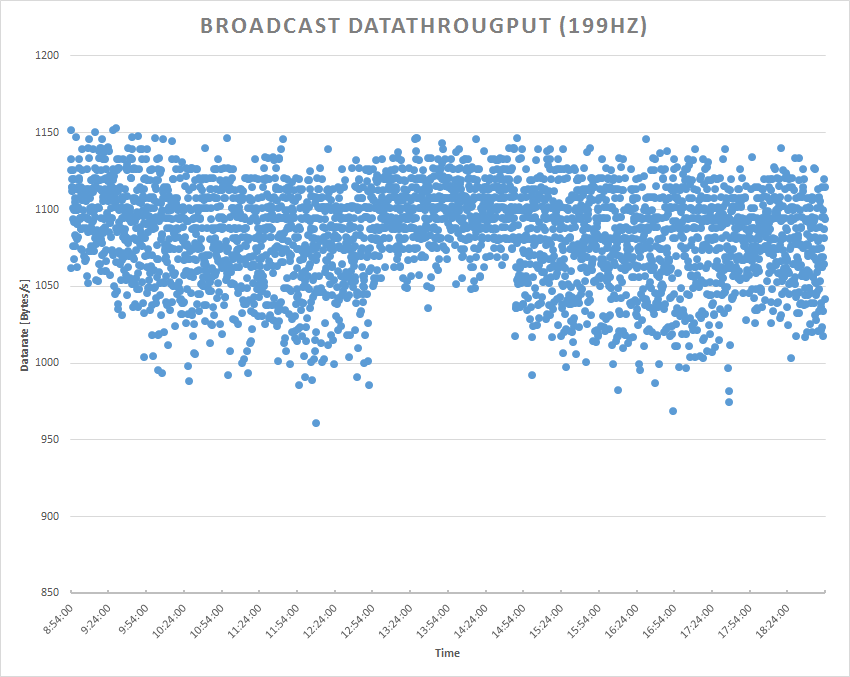
\includegraphics[scale=0.5]{./pics/exp1_long.png}
		\caption{Broadcast data rate over time (200Hz)}\label{fig:exp1long}
	\end{figure}
	Figure \ref{fig:exp1long} shows the transmission speed for the highest supported frequency 199.8 Hz over time. The results show that the data throughput stays fairly consistent with a standard deviation of only 30 Bps, or 2.7\%. Interesting to note is the time period from 1:00PM to 2:50 PM, where the deviation from the average is much smaller. The exact reason for this phenomenon in unknown, since during this time period the environment of the test set up did not change in any way.
\end{description}
\newpage

\section{Experiment 2: Broadcast Data Transfer between multiple nodes}
\begin{description} 
	\item{\textbf{Description}} \hfill \\ In experiment 1 we determined the channel period, which allows for the maximum throughput. In this experiment we try to determine, how the maximum throughput is affected by the amount of channels in the network. SHAMPU needs two channels, so it can work correctly: One channel which sends data from the base station to the nodes in order to control them and another channel by which the nodes can send debugging and other information.
	\item{\textbf{Use-Case}} \hfill \\ Scheduled Data-transmission	
	\item{\textbf{Network Topology and Configuration}} \hfill
		\begin{figure}[H]
			\centering
			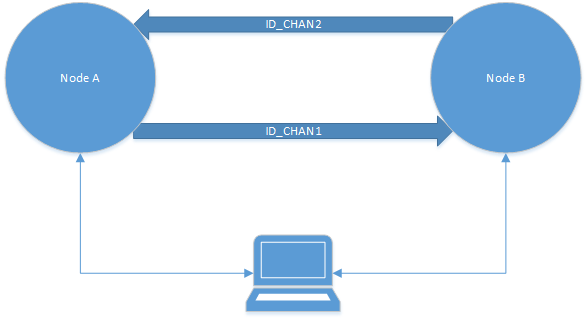
\includegraphics[scale=1]{./pics/exp2_topo.png}
			\caption{Toplogy experiment 2}
		\end{figure}
		\begin{code}[H]
			\begin{verbatim}
			channelPeriod = max_Channel_Period
			while (channelPeriod >= min_Channel_Period) {
			  ANT_SetChannelPeriod(ID_CHAN1, channelPeriod)
			  openChannel(ID_CHAN1, ANT_Bidirectional_Master)
			  ANT_SendBroadcastData(ID_CHAN1, [0x01, 0x02, 0x03, 0x04])
			  ANT_SetChannelPeriod(ID_CHAN2, channelPeriod)
			  openChannel(ID_CHAN2, ANT_Bidirectional_Slave)
			  count = 0
			  for (10 seconds) 
			    if (receivedPacket() == ANT_BROADCAST_DATA)
			    count++			
			  print (count * 8 / 10) + " Bytes per second"
			  wait_for_user_input()
			  ANT_CloseChannel(ID_CHAN1)
			  ANT_CloseChannel(ID_CHAN2)
			  channelPeriod = decreaseChannelPeriod()
			}
			\end{verbatim}
			\caption{Broadcast data transfer two channels (Master)}\label{lst:mExp2}
		\end{code}
		
		\begin{code}[H]
			\begin{verbatim}
			channelPeriod = max_Channel_Period
			while (channelPeriod >= min_Channel_Period) {
			  ANT_SetChannelPeriod(ID_CHAN1, channelPeriod)
			  openChannel(ID_CHAN1, ANT_Bidirectional_Slave)
			  ANT_SetChannelPeriod(ID_CHAN2, channelPeriod)
			  openChannel(ID_CHAN2, ANT_Bidirectional_Master)
			  ANT_SendBroadcastData(ID_CHAN2, [0x01, 0x02, 0x03, 0x04])
			  count = 0
			  for (10 seconds) 
			    if (receivedPacket() == ANT_BROADCAST_DATA)
			      count++			
 			  print (count * 8 / 10) + " Bytes per second"
			  wait_for_user_input()
			  ANT_CloseChannel(ID_CHAN1)
			  ANT_CloseChannel(ID_CHAN2)
			  channelPeriod = decreaseChannelPeriod()
			}
			\end{verbatim}
			\caption{Broadcast data transfer two channels (Slave)}\label{lst:mExp2}
		\end{code}
 
	\item{\textbf{Network Topology and Configuration}} \hfill \\ The two nodes are placed right next to each other.
	\item{\textbf{Testing methodology}} \hfill \\ In this experiment each node acts as a master for a different channel. Node A is the master for Channel 0 and Node B is the master for Channel 1. The measurements itself are identical to the ones in experiment 1, except that the data is recorded on both nodes. The channel period is decreased until the data throughput decreases, or the connection can no longer be established.
	\item{\textbf{Result}} \hfill \\  	
	\begin{figure}[H]
		\centering
		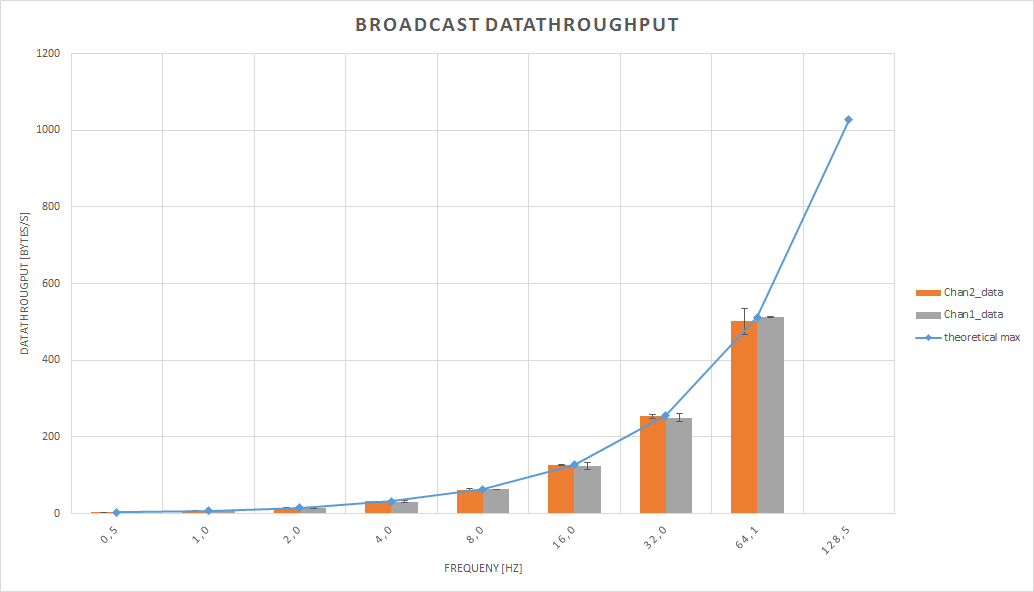
\includegraphics[scale=0.5]{./pics/exp2_norm.png}
		\caption{Broadcast data through - 2 channels (0.5Hz - 129Hz)}\label{fig:exp2low}
	\end{figure}
	\begin{figure}[H]
		\centering
		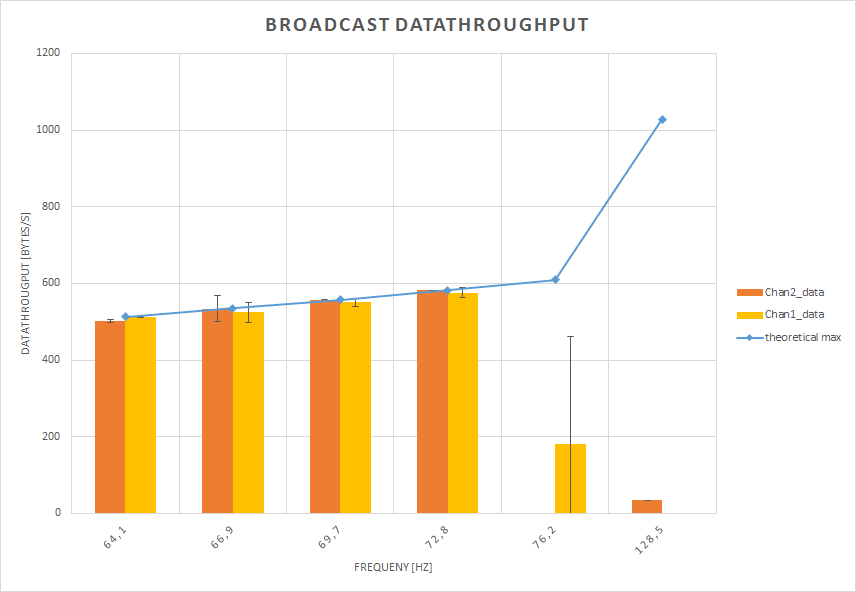
\includegraphics[scale=0.5]{./pics/exp2_detail.png}
		\caption{Broadcast data through - 2 channels (64Hz - 129Hz)}\label{fig:exp2high}
	\end{figure}
	Figures \ref{fig:exp2low} shows the results of the measurements, the left bar displaying the throughput for channel 0, the right bar displaying the throughput for channel 1. The blue line shows the theoretical maximum of the data throughput for the given frequency. Up to a frequency of 64 Hz the data throughput increases with the frequency for both channels. However there is a complete drop at 128 Hz. Figure \ref{fig:exp2high} shows that somewhere between 72 Hz and 76 Hz the data throughput begins to drop off. The maximum combined data rate for two channels adds up to around 1160 Bps, which is in line with the result from experiment 1. From this data we can assume, that the entire available data rate of 1160 Bps is simply split among all existing channels.
\end{description}
\newpage


\section{Experiment 3: Acknowledge Transfer delay}
\begin{description} 
	\item{\textbf{Description}} \hfill \\ In this experiment we try to determine the time it takes for a node to receive and acknowledge a transmitted packet. The value is important in order to be able to determine the reaction time of SHAMPU to commands sent by the base station, for example to set up a separate channel for a burst transmission.
	\item{\textbf{Use-Case}} \hfill \\ Scheduled Data-transmission
	\item{\textbf{Network Topology and Configuration}} \hfill \\ 
	\begin{figure}[H]
		\centering
		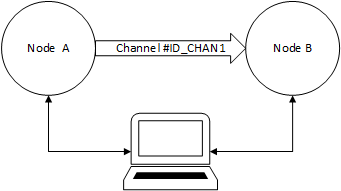
\includegraphics[scale=1]{./pics/exp_topo.png}
		\caption{Toplogy experiment 3}
	\end{figure}
	\begin{code}[H]
		\begin{verbatim}
		channelPeriod = max_Channel_Period
		while (channelPeriod >= min_Channel_Period) {
		  ANT_SetChannelPeriod(ID_CHAN1, channelPeriod);
		  ANT_OpenChannel(ID_CHAN1, ANT_Bidirectional_Master);
		  duration = 0.0
		  for (i in 0..10) {
		    ANT_SendAcknowledgedData(ID_CHAN1, [0x01, 0x02, 0x03, 0x04])
		    start = getTime()	   
		    wait_for_ack()		
		    print (getTime() - start) + " s"	  
		  }
		  ANT_CloseChannel(ID_CHAN1)		
		  channelPeriod = decreaseChannelPeriod()
		} 
		\end{verbatim}
		\caption{Acknowledge data delay (Master)}\label{lst:mExp3}
	\end{code}
	
	\begin{code}[H]
		\begin{verbatim}
		channelPeriod = max_Channel_Period
		while (channelPeriod >= min_Channel_Period) {
		  ANT_SetChannelPeriod(ID_CHAN1, channelPeriod);
		  ANT_OpenChannel(ID_CHAN1, ANT_Bidirectional_Slave);				 
		  wait_for_user_input();
		  ANT_CloseChannel(ID_CHAN1);
		  channelPeriod = channelPeriod >> 1;
		}
		\end{verbatim}
		\caption{Acknowledge data delay (Slave)}\label{lst:sExp3}
	\end{code}
	
	\item{\textbf{Testing methodology}} \hfill \\ Node A acts as the master and node B as the slave. For both nodes the channel period is set to the highest value and the channel is opened. Node A then sends a total of 10 acknowledge messages and measures how long it takes until it receives the acknowledge signal. The channel period is then decreased and the experiment repeated.
	\item{\textbf{Result}} \hfill \\  
	\begin{figure}[H]
		\centering
		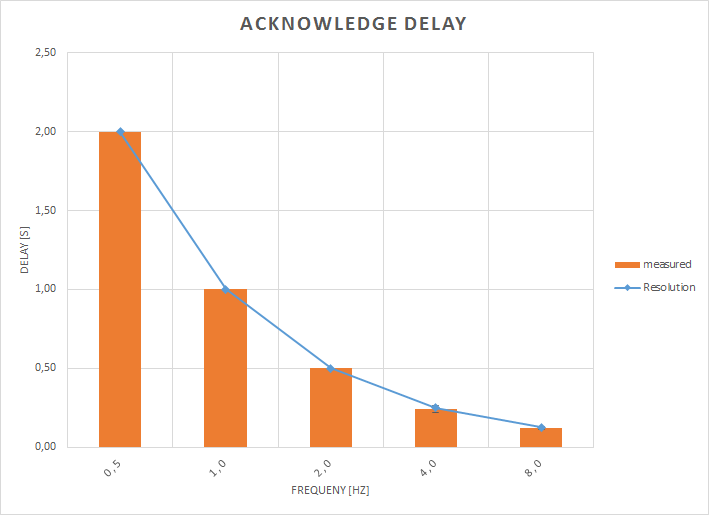
\includegraphics[scale=0.5]{./pics/exp3_norm.png}
		\caption{Acknowledge delay (0.5Hz - 8Hz)}\label{fig:exp3low}
	\end{figure}
	\begin{figure}[H]
		\centering
		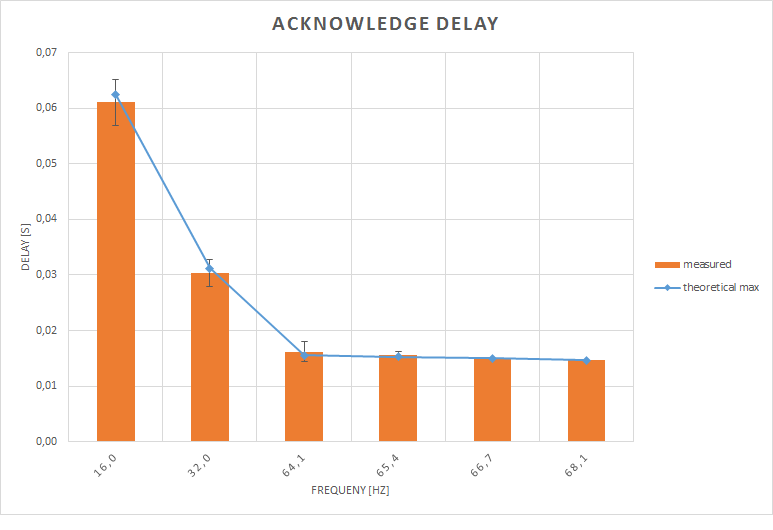
\includegraphics[scale=0.5]{./pics/exp3_detail.png}
		\caption{Acknowledge delay (16Hz - 70Hz)}\label{fig:exp3high}
	\end{figure}
	Figure \ref{fig:exp3low} and \ref{fig:exp3high} show the delays for the tested frequencies. The blue line shows the size of the gap between two timeslots and can act as a resolution for each measurement. For the lower frequencies the results are skewed, since each acknowledge packet is aligned to a time-slot. Thus the biggest part of the delay is waiting for the next time-slot. For frequencies greater than 64 Hz the data is considerably more useful, since the resolution is lower than the measured values. The delay for those frequencies is around 18 ms, with no notable difference between 128 Hz and 200 Hz. Since the procedure is the same for the higher channel periods, it can be assumed that the delay is the same as the one for the lower channel periods.
\end{description}
\newpage


\section{Experiment 4: Acknowledge Data Transfer between two nodes}
\begin{description} 
	\item{\textbf{Description}} \hfill \\ This experiment is almost identical with experiment 1. The main difference is that we use acknowledge data instead of broadcast. It is also important to note that the master records how many successful packets are transmitted. The main goal of the experiment is to see if the data throughput is decreased compared to broadcast data, especially for smaller channel periods.
	\item{\textbf{Use-Case}} \hfill \\ Scheduled Data-transmission
	\item{\textbf{Network Topology and Configuration}} \hfill \\
	\begin{figure}[H]
		\centering
		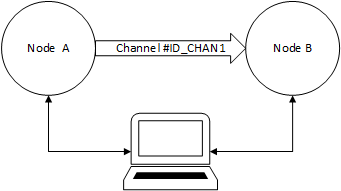
\includegraphics[scale=1]{./pics/exp_topo.png}
		\caption{Toplogy experiment 4}
	\end{figure}
	\begin{code}[H]
		\begin{verbatim}
		channelPeriod = max_Channel_Period
		while (channelPeriod >= min_Channel_Period) {
		  ANT_SetChannelPeriod(ID_CHAN1, channelPeriod)
		  ANT_OpenChannel(ID_CHAN1, ANT_Bidirectional_Master)
		  count = 0
		  for (10 seconds) {
		    ANT_SendAcknowledgedData(ID_CHAN1, [0x01, 0x02, 0x03, 0x04])	   
		    wait_for_ack()
		    count++
		  }
		  print (count * 8 / 10) + " Bytes per second"	  
		  ANT_CloseChannel(ID_CHAN1)
		  channelPeriod = decreaseChannelPeriod()
		} 
		\end{verbatim}
		\caption{Acknowledge data transfer (Master)}\label{lst:mExp4}
	\end{code}
			
	\begin{code}[H]
		\begin{verbatim}
		channelPeriod = max_Channel_Period
		while (channelPeriod >= min_Channel_Period) {
		  ANT_SetChannelPeriod(ID_CHAN1, channelPeriod)
		  ANT_OpenChannel(ID_CHAN1, ANT_Bidirectional_Slave)
		  wait_for_user_input()
		  ANT_CloseChannel(ID_CHAN1)
		  channelPeriod = channelPeriod >> 1
		}
		\end{verbatim}
		\caption{Acknowledge data transfer (Slave)}\label{lst:sExp4}
	\end{code}
	\item{\textbf{Testing methodology}} \hfill \\ The testing methodology is the same as experiment 1a, except that the master sends acknowledge messages and waits for the slave to confirm the successful transmission before sending the next packet. 
	\item{\textbf{Result}} \hfill \\
	\begin{figure}[H]
		\centering
		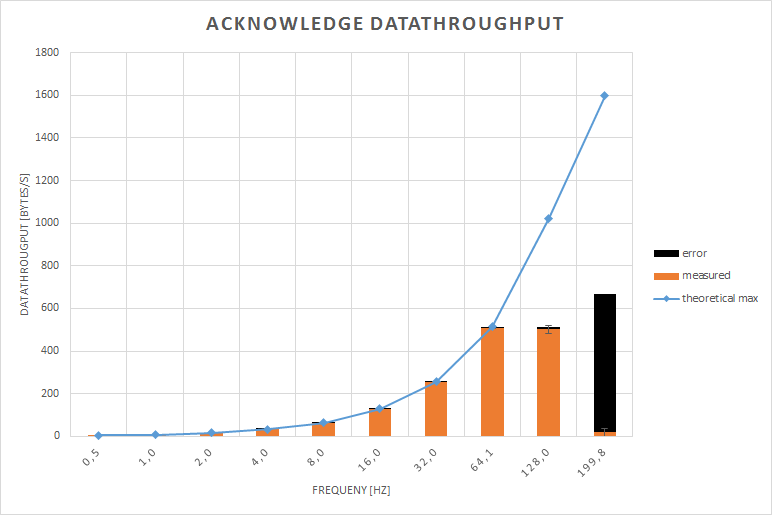
\includegraphics[scale=0.5]{./pics/exp4_norm.png}
		\caption{Acknowledge data rate (0.5Hz - 129Hz)}\label{fig:exp4norm}
	\end{figure}
	\begin{figure}[H]
		\centering
		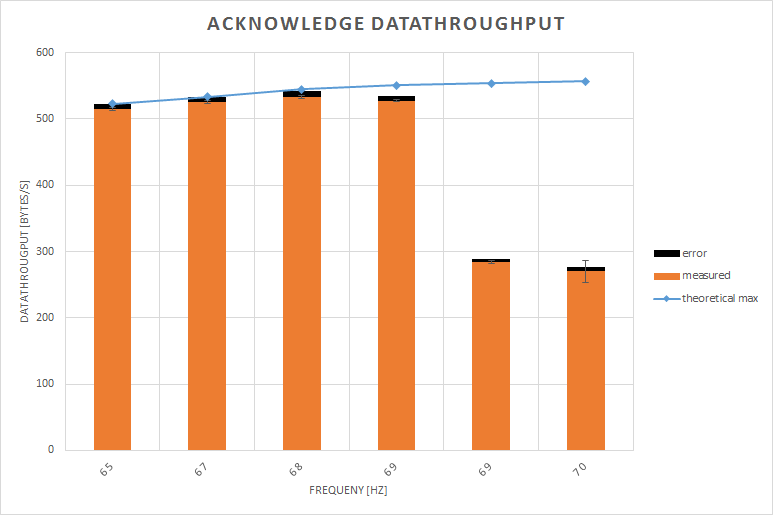
\includegraphics[scale=0.5]{./pics/exp4_detail.png}
		\caption{Acknowledge data rate (65Hz - 70Hz)}\label{fig:exp4between}
	\end{figure}
	
	Figure \ref{fig:exp4norm} shows the measured transmission speeds for the different tested frequencies. For the lower frequencies, the values align very well with the maximum data rate. Notable however is the sharp drop off at 129 Hz. Figure \ref{fig:exp4between} shows
	that the drop off in the data throughput rate starts around 69 Hz. This result can be explained with the results of experiment 3. The delay of an acknowledge message is roughly 18 ms. The problem is that ANT retransmits the last sent packet as a broadcast packet. If the frequency for this retransmission is too high it can interfere with the acknowledge message that the slave sends back to the master. For example at 200 Hz the message is broadcast every 5 ms, resulting in too much data for the channel to handle. The transmission is thus interrupted. Since there is no increase of the data throughput between 64 Hz and 128 Hz, but a huge drop off at 69 Hz it can be assumed that somewhere around 69 Hz the channel is at the maximum data throughput of around 1100 Bps. Again see section \ref{sec:dataThrougput} for a discussion about possible reasons for this upper limit. 

\end{description}
\newpage

\section{Experiment 5: Burst Data Transfer between two nodes}
\begin{description} 
	\item{\textbf{Description}} \hfill \\ Burst data transmissions make it possible to drastically increase the throughput rate. This allows a SHAMPU base station to quickly transmit a new firmware to a node or a node to dump its RAM back to the base station.	According to the  specification rates of up to 20 kbps can be achieved. To fully utilize this speed a baud rate of 50000 is needed. Since we are using 19200 baud the maximum speed is expected to be less than 20 kbps. Furthermore we try to determine if the size of the burst transfer has an impact on the speed, since longer bursts will disrupt communications on other channels.
	\item{\textbf{Use-Case}} \hfill \\ Unscheduled Data-transmission
	\item{\textbf{Network Topology and Configuration}} \hfill \\ 
	\begin{figure}[H]
		\centering
		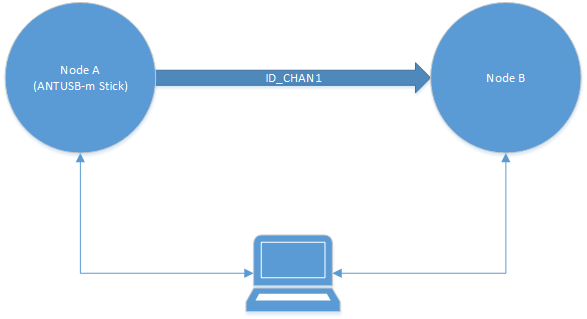
\includegraphics[scale=1]{./pics/exp5_topo.png}
		\caption{Toplogy experiment 5}
	\end{figure}
	\begin{code}[H]
		\begin{verbatim}
		size = START_SIZE
		ANT_OpenChannel(ID_CHAN1, ANT_Bidirectional_Slave);		
		while (size >= END_SIZE) {
		  for (i in 0..10) {
		    wait_for_first_burst_packet()
		    start = getTime()
		    wait_for_last_burst_packet()
		    print (getTime() - start) / (size - 1) " Bytes per second"
		  }
		  size = 2 * size
		}
		\end{verbatim}
		\caption{Burst data transfer (Slave)}\label{lst:sExp5}
	\end{code}
	\item{\textbf{Testing methodology}} \hfill \\ Since the burst transmission mode of our ANT-library is not working correctly (see section \ref{sec:future}) we use an ANTUSB-m Stick, which acts as a master. Node B is a normal base station and receives the burst transfers. On the master side, the program ANTWareII \cite{ANTwareII} is used to create the channel and then send bursts with different sizes. Each size is sent 10 times and the values are recorded and averaged. The size is then doubled and the experiment repeated. The first burst packet cannot be counted directly since the start of the burst can only be determined after the ANT chip has already received the first packet.
	\item{\textbf{Result}} \hfill \\ 
		\begin{figure}[H]
			\centering
			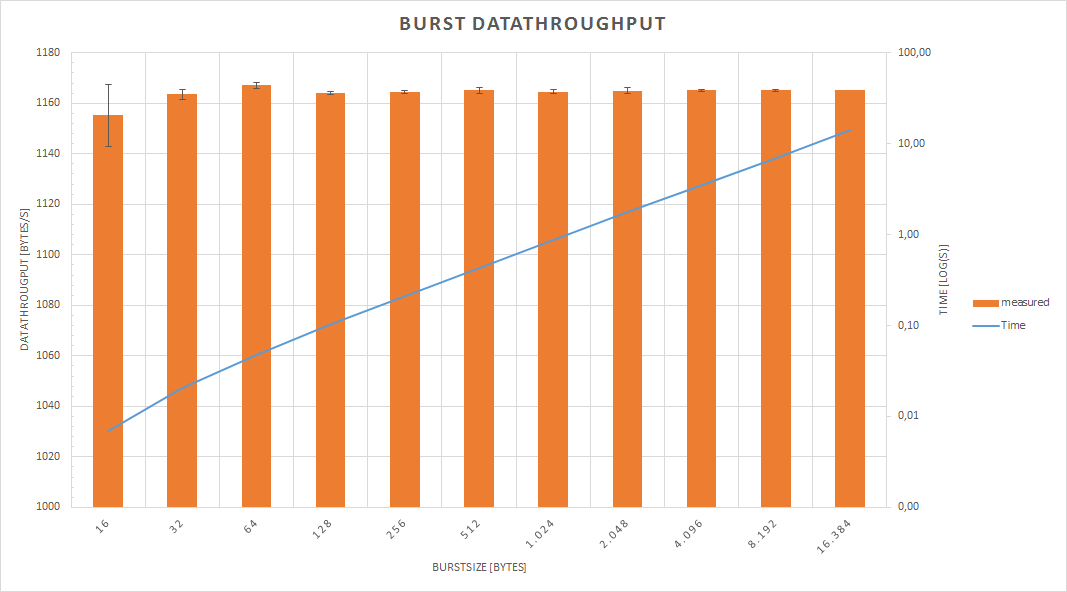
\includegraphics[scale=0.5]{./pics/exp5.png}
			\caption{Burst data rate}\label{fig:exp5}
		\end{figure}
	 Figure \ref{fig:exp5} shows the achieved data rates for the different packet sizes and also the length of the transfer. As seen the values all hover around the same value of ~1165 Bps. This is approximately the same value as the one which can be achieved with the other two types of data.
	 Again see section \ref{sec:dataThrougput} for a discussion about possible reasons for this upper limit. 
\end{description}
\newpage

\section{Experiment 6: Maximum communication Range}
\begin{description} 
	\item{\textbf{Description}} \hfill \\  In this experiment we try to determine the correlation between the maximum range and the power setting of the ANT radio. One of SHAMPU's advantages is the low power consumption, so it might be possible to further reduce the power consumption by decreasing the power level of the ANT radio, especially in smaller environments where there is no need for such a long range. According to the datasheet the maximum range for communication is 30m. However the ANT documentation does not specify for which power setting this range can be achieved. 

	\item{\textbf{Use-Case}} \hfill \\ Communication Range		
	\item{\textbf{Network Topology and Configuration}} \hfill \\ 
	\begin{figure}[H]
		\centering
		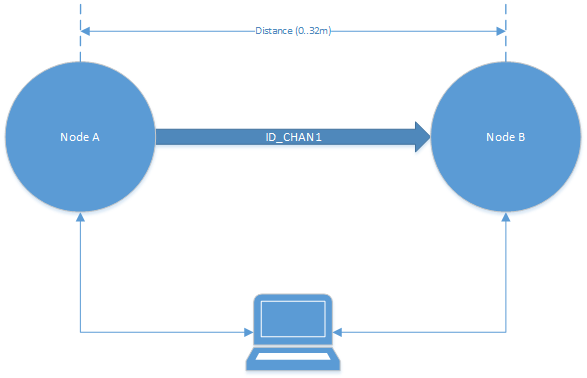
\includegraphics[scale=1]{./pics/exp6_topo.png}
		\caption{Topology experiment 6}
	\end{figure}
	
	\begin{code}[H]
		\begin{verbatim}
		for (pSetting in Available_PowerSettings) {
		  ANT_SetTransmitPower(pSetting)
		  openChannel(ID_CHAN1, ANT_Bidirectional_Master)
		  ANT_SendBroadcastData(ID_CHAN1, [0x01, 0x02, 0x03, 0x04])
		  wait_for_user_input();
		  closeChannel(ID_CHAN1);
		}
		\end{verbatim}
		\caption{maximum communication range (Master)}\label{lst:mExp6}
	\end{code}
	
	\begin{code}[H]
		\begin{verbatim}
		distance = 0.0
		stopInc = false
		loop {
		  openChannel(ID_CHAN1, ANT_Bidirectional_Slave)
		  wait_until(received_Packet == ANT_BROADCAST_DATA || 
		             received_Packet == ANT_MESSAGE_EVENT_RX_SEARCH_TIMEOUT) {
		    if (stopInc) { 
		      if (wasTimeout) distance -= .4
		      else print "Connection found : " + distance
		    } else {
		      if (wasTimeout) { 
		        stopInc = true; distance -= .54
		        print "Connections lost : " + distance
		      } else distance += .4
		    }
		  }
		  closeChannel(ID_CHAN1);		
		}
		
		\end{verbatim}
		\caption{maximum communication range (Slave)}\label{lst:sExp6}
	\end{code}
	\item{\textbf{Testing methodology}} \hfill \\ At the beginning of the experiment Node A and B are placed right next to each other. Node A acts as a master and keeps broadcasting the same message. Node B is the slave and tries to connect to the channel. If the connection is successful, the distance between the two nodes is increased by 0.4 meters. This process is repeated until Node B can no longer connect to the channel and the connection times out. This happens after 30s of searching. At this point the distance is no longer increased, but rather decreased until Node B is able to successfully connect to the channel. The whole experiment is then repeated for each available power setting.	
	\item{\textbf{Result}} \hfill \\ 
	\begin{figure}[H]
		\centering
		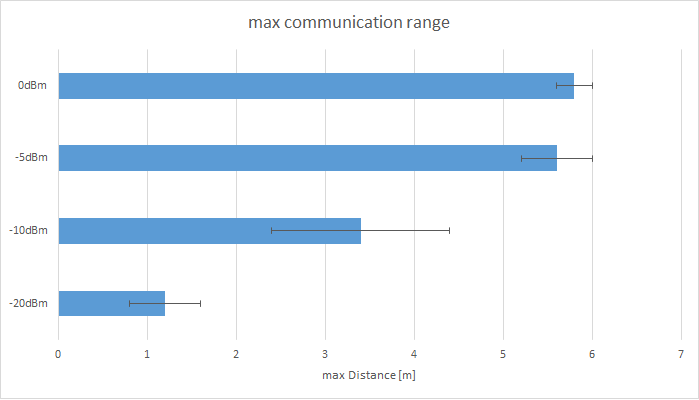
\includegraphics[scale=0.5]{./pics/exp6.png}
		\caption{maximum comunication range}\label{fig:exp6}
	\end{figure}
	Figure \ref{fig:exp6} shows the transmission range for each power setting. As expected the maximum distance goes up with the higher power settings. But the result at the highest power setting is disappointing, since we did not get close to the claimed maximum range of 30m. The ANT documentation states that the maximum range of 30m can only be achieved in "optimal conditions"\cite{DynastreamInnovationsInc.2013}. It is possible for several different unfavourable factors, such as multiple 802.11 networks in the vicinity, or even the plastic case of the base station, to interfere with the ANT signal. 
\end{description}
\newpage


\chapter{Conclusion}

\section{Maximum Data Throughput}
\label{sec:dataThrougput}

All our experiments seem to confirm that there is a hard limit for the maximum data throughput which can be achieved with our current set up. The ANT AP1MxIB supports a maximum frequency of 200 Hz, so we would expect to see a maximum transmission rate of 1600 Bps. However, we missed that limit by around 500 Bps or 30\%. For a burst transmission there should be up to 20 kbps of throughput, but again we only achieved around 1100 Bps, a loss of 1400 Bps or 56\%.\\
To eliminate environmental influences, the experiments were repeated in different locations and times of day and night. Since the throughput did not change noticeably, it can be assumed that there are no easily eliminated environmental factors which affect the maximum rate. We conclude that the root cause for the lower than expected throughput must be attributed to the hardware or software. \\

If we exclude environmental factors, we are left with three possible reasons:
\begin{itemize}
	\item{\textbf{RS-232 Connection}} \hfill \\ The base station is connected to a PC over a serial connection. For the speed we chose 19200 baud, which should be more than enough for a maximum message rate of 200 Hz. For the burst mode however, this is one limiting factor. With 19200 baud, the theoretical maximum is 1920 Bps. This explains some, but not all of the measured difference.
	
	\item{\textbf{ANT API}} \hfill \\ The software we use is not officially supported by ANT. It is thus possible that there are some bugs which have an impact on the performance. Except for the missing burst modus (see \ref{sec:future}), there were no unusual measured values during the experiments. If there is a bug, it might be hard to find without rewriting all the experiments and running them with the official ANT library \cite{ANTWinLib}
	
	\item{\textbf{ANT AP1MxIB}} \hfill \\ Due to the black box nature of ANT, it is very hard to exactly determine what causes the problem. The inner workings of the chip are not documented in any way, and the error messages of the protocol are not very specific. The chip itself is from 2007 and the manufacturer no longer recommends the use of the chip\cite{AP1page}. There are alternatives available, like the newer ANTAP281M5IB chip \cite{AP2Datasheet}.
\end{itemize}
\newpage
\section{Summary}
In conclusion of our experiments, it seems af if the ANT chip falls short of its full potential:
\begin{itemize}
	\item{\textbf{Scheduled data-transmission}} \hfill \\ The achieved data throughput of around 1160 Bps is valid for a single chip. That means the main bottleneck of the network is the base station, since it acts as a command and control server for each node in the network. The easiest way to fix the problem is to use more than one base station. This is possible, since we do not need a fully meshed network for the SHAMPU nodes to communicate with each other. They solely need to talk to the base station.
	
	\item{\textbf{Unscheduled data-transmission}} \hfill \\ The achievable burst data throughput is especially problematic. SHAMPU is equipped with 128 kBytes of RAM. With the current set up it takes about 2 minutes to dump the entire memory to a base station, where is can be further analysed. If the full potential of the burst mode could be made available, the duration can be shortened to 70s. The long burst duration poses a problem, as long bursts disrupt the communication on other channels. For this reason the transmission of these memory-dumps has to be very carefully scheduled to avoid network congestion.
	
	\item{\textbf{Communication Range}} \hfill \\ The maximum achieved range of 6m is probably the most disturbing result of this thesis. The short range signifies, that the physical location of the base station is critical for a successful deployment of SHAMPU. It also means that a larger network requires more than one such base station to be able to reach all nodes.
\end{itemize}


With all these limitations of the data throughput, the network setup has to be chosen very carefully. One option is to use additional SHAMPU nodes as relays, which serve a dual purpose. They allow to extend the range of the network, while increasing the data throughput of the whole network.\\ Another possibility to counteract the limitation is to leverage the numerous advantages of the SHAMPU framework, such as its low weight, form factor and power draw. A mobile base station, e.g. TrainSense \cite{Smeets:2013:TNI:2450070.2450072}, which can easily be moved around in the location where the SHAMPU nodes are deployed, makes it possible to address all above mentioned problems. The range no longer represents a problem, since the base station is simply moved towards the node until a connection can be achieved. At the same time, the limited range provides a solution for the limited data throughput. Since the amount of nodes, which are able to connect to the base station can be controlled its possible to only ever have a small number of nodes transmitting data to the base station.

In the end, while ANT is not the most powerful wireless solution available, its design choices (low power consumption and ease-of-use) coincide almost completely with the design goals of SHAMPU.
\newpage
\section{Future Work}
\label{sec:future}
Due to lack of time and the limited hardware availability we were not able to fully explore and evaluate the possibilities of ANT in the SHAMPU network. Especially the following four areas should be revisited:

\begin{itemize}
	\item{\textbf{Power consumptions}} \hfill \\ Each experiment tries to find the maximum of either data throughput or the communication range. We did not measure how the power consumption changes if, for example, the message period is reduced. Since SHAMPU tries to be very low-powered, this is an important measurement for the decision whether or not SHAMPU can be used for a specific application. The data sheet of the ANT AP1MxIB module provides interesting data \cite{Networks}: The maximum current draw seems to be around 5 mA for a continuous burst transmission and around 40 µA for a normal broadcast operation.
	
	\item{\textbf{Burst mode}} \hfill \\ We use a custom library, which provides an API to interface with the ANT-Chip. For this thesis an attempt was made to add the missing burst transfer mode. However, due to time constraints we were unable to get the mode working correctly. Burst packets need to have a precise timing, but the black box nature of the ANT protocol makes it a challenge to debug the code.
	
	\item{\textbf{Shared channels}} \hfill \\ Due to missing hardware, we were only able to test the communication between two nodes. Shared channels could not be tested, yet we expect the available data throughput to be in line with the results from our experiments. ANT uses up to 2 bytes of the 8 byte payload to specify the address of the receiver. Therefore we expect to lose approximately 12.5\% to 25\% of throughput if shared channels are used. It would be important to confirm this to fully assess the usefulness of the ANT chip.
	
	\item{\textbf{New ANT-chip}} \hfill \\ As mentioned before the chip currently in use is old and no longer recommended for use. The successor of the current chip, the ANTAP281M4IB has roughly the same specifications as the current chip. Therefore the experiments should be rerun with the newer model in order to determine whether the ANT-chip is the limiting factor for data throughput.
\end{itemize}